\begin{figure}[t]
    \centering
    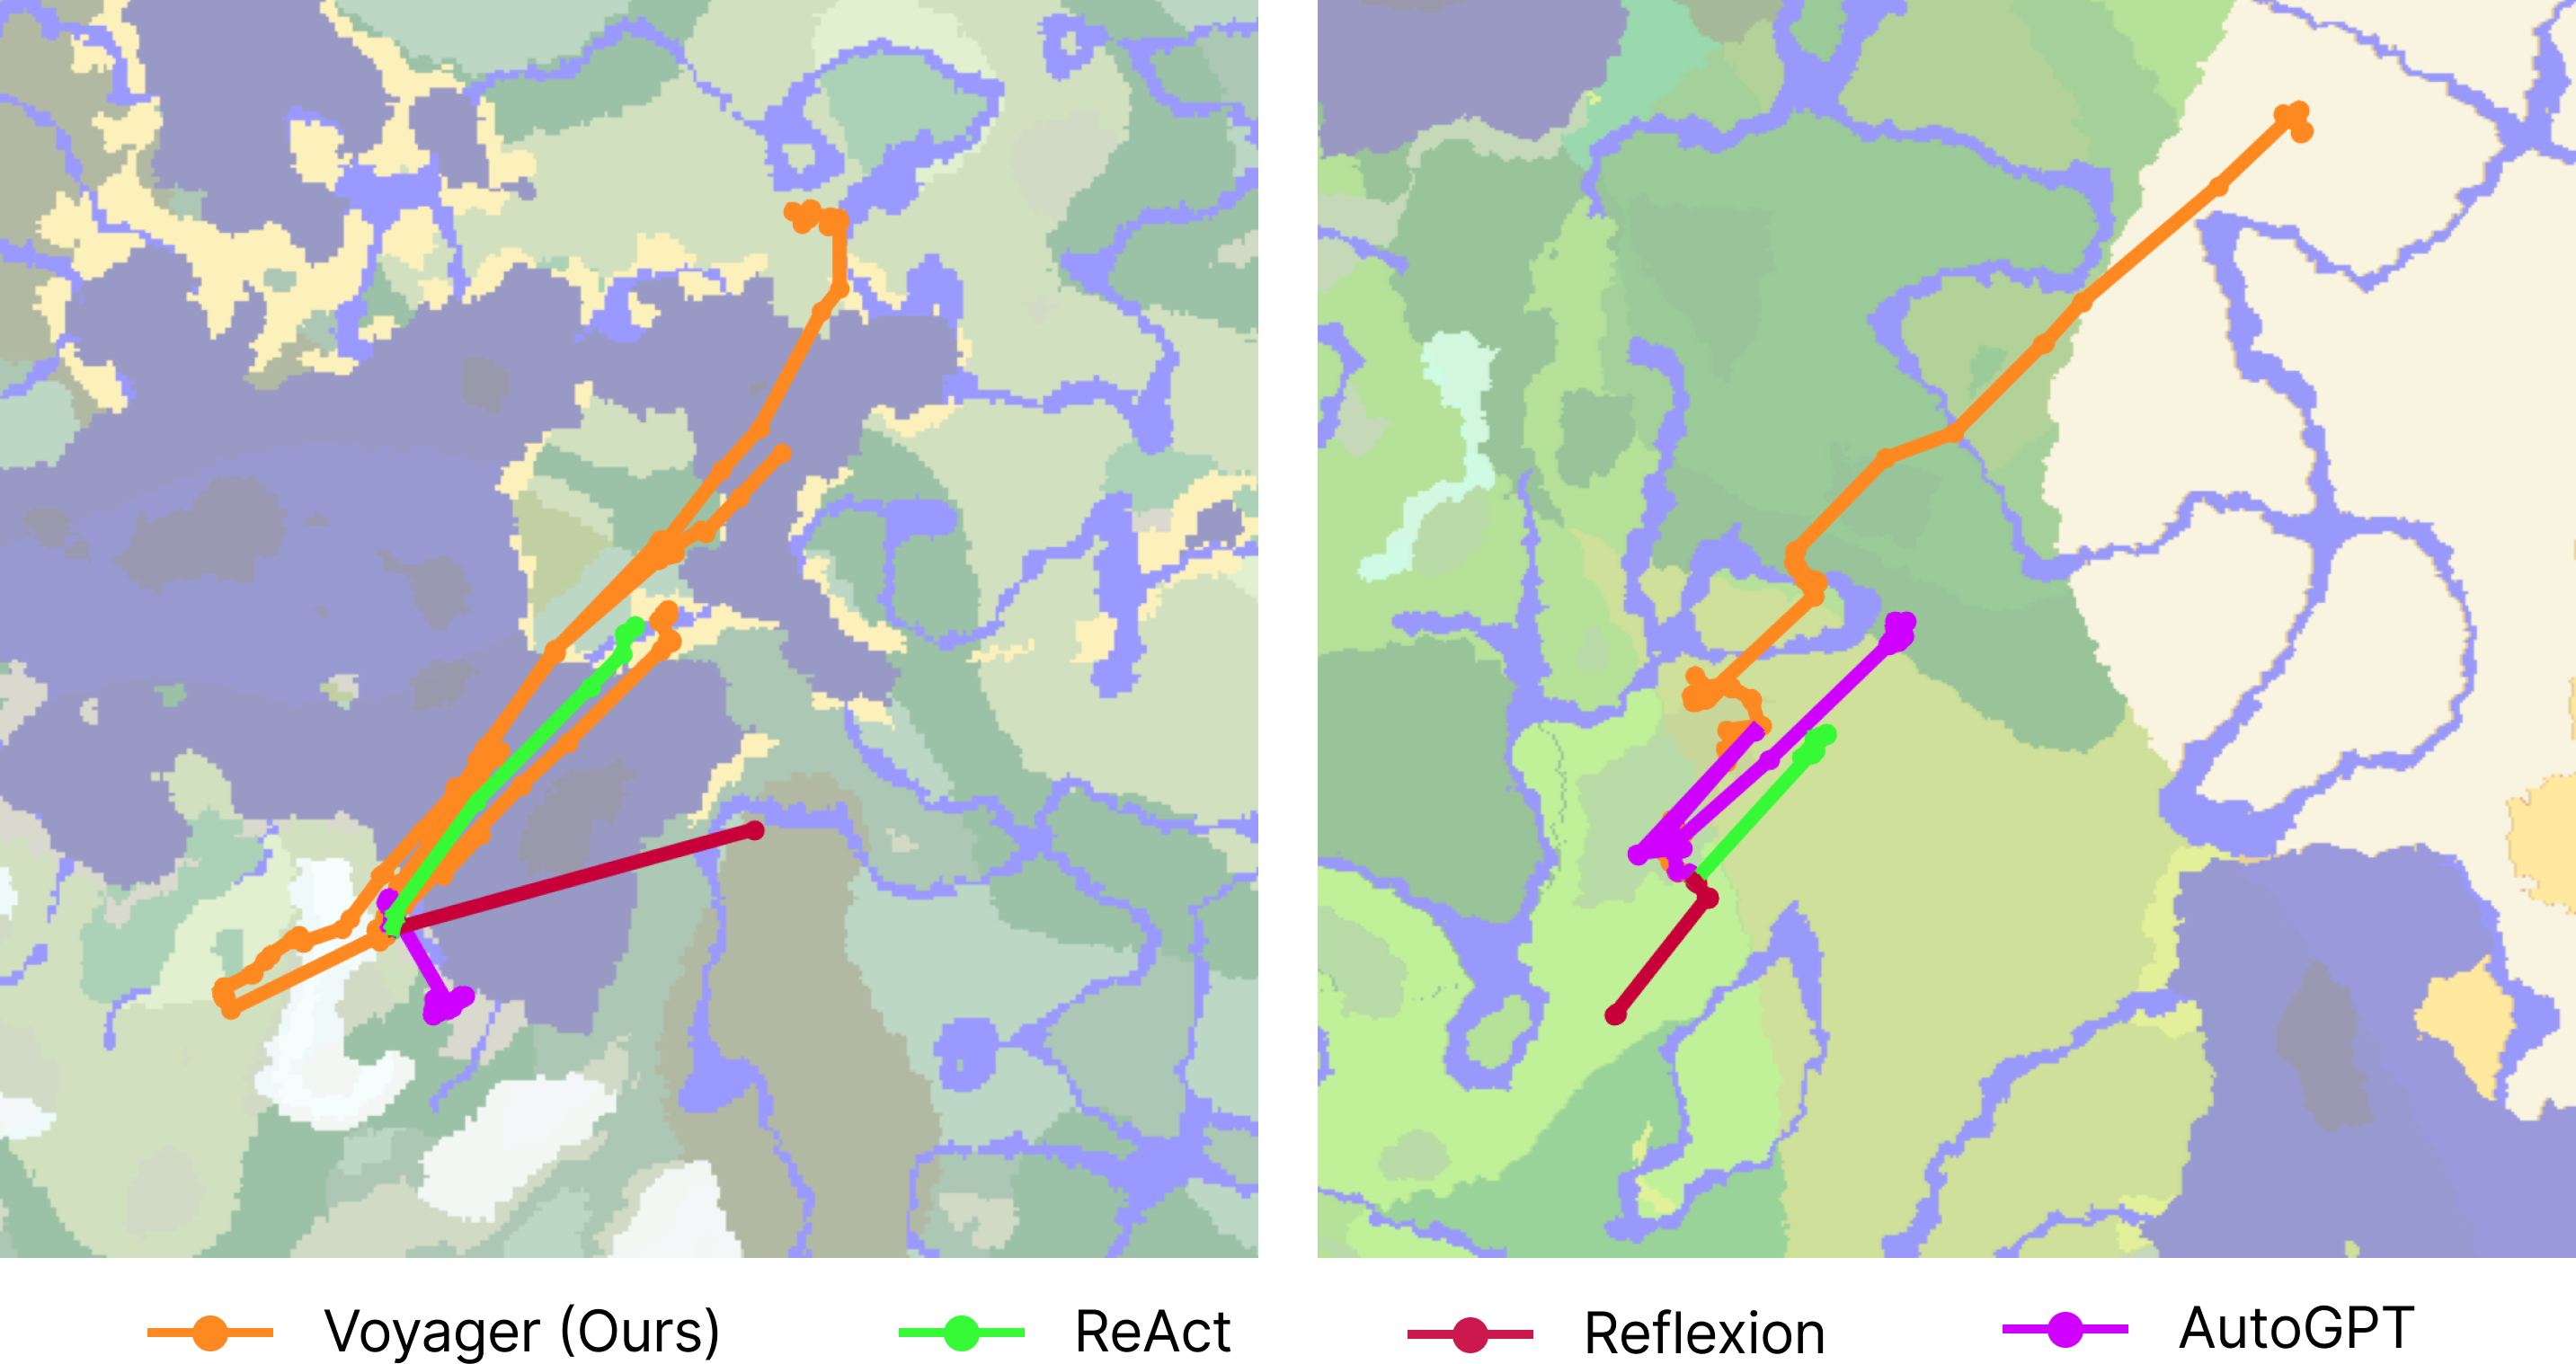
\includegraphics[width=\textwidth]{appendix/figures/map_traj_fig.png}
    \vspace{0.05em}
    \caption{Map coverage: Two bird's eye views of Minecraft maps. \voyager is able to traverse $2.3 \times$ longer distances compared to baselines while crossing diverse terrains. Trajectories are plotted based on the positions where each agent interacts with GPT-4.}
    \label{supp:fig:map}
    \vspace{-1em}
\end{figure}